\documentclass[11pt,a4paper]{article}
\usepackage[T1]{fontenc}
\usepackage[utf8]{inputenc}
\usepackage{lmodern,amsmath,amssymb,amsthm,mathtools,microtype}
\usepackage[margin=26mm]{geometry}
\usepackage{graphicx,booktabs,array}
\usepackage[dvipsnames]{xcolor}
\usepackage[colorlinks=true,linkcolor=MidnightBlue,citecolor=MidnightBlue,urlcolor=MidnightBlue]{hyperref}
\hypersetup{pdftitle={Hidden architecture and the thermodynamic cost of an exact stochastic signal},pdfauthor={Anonymous},pdfsubject={Exact hidden Markov realisation and entropy-production optimisation},pdfkeywords={stochastic thermodynamics, hidden Markov models, phase-type distributions, entropy production}}
\usepackage{fancyhdr}
\pagestyle{fancy}\fancyhf{}
\fancyhead[L]{\small Hidden architecture and dissipation}
\fancyhead[R]{\small Evidence Press research candidate v1.0}
\fancyfoot[C]{\thepage}
\setlength{\headheight}{14pt}
\setlength{\parskip}{3pt}
\newtheorem{theorem}{Theorem}
\newtheorem{proposition}[theorem]{Proposition}
\newtheorem{lemma}[theorem]{Lemma}
\newtheorem{corollary}[theorem]{Corollary}
\theoremstyle{remark}\newtheorem{remark}[theorem]{Remark}
\newcommand{\one}{\mathbf 1}
\newcommand{\R}{\mathbb R}
\newcommand{\atanh}{\operatorname{artanh}}
\newcommand{\diag}{\operatorname{diag}}
\newcommand{\Exp}{\operatorname{Exp}}
\newcommand{\J}{\mathcal J}
\title{Hidden architecture and the thermodynamic cost\newline of an exact stochastic signal}
\author{}
\date{Anonymous\\[2pt]\small Evidence Press research candidate, version 1.0.0-candidate, 28 October 2026\\\small DOI \href{https://doi.org/10.5281/zenodo.23721621}{10.5281/zenodo.23721621}}
\begin{document}
\maketitle
\thispagestyle{empty}
\begin{abstract}
When only part of a system can be watched, one model-based way to bound its
dissipation is to fit the smallest hidden Markov model that explains the data
and minimise entropy production over that model. We show by an exact
example that this procedure can overstate the least possible dissipation,
even when the observed signal is known perfectly.
We prove that increasing the number of hidden states can strictly reduce the
least entropy production compatible with an entire observed stochastic process.
For a binary alternating-renewal family, we determine the global minimum over
all three-state continuous-time Markov realisations: the homogeneous driven ring
is the unique minimiser up to relabelling, with cost $(1-q)\log(1/q)$.
For every $0<q<1$, we construct a finite four-state exact realisation with
strictly smaller cost. At $q=1/20$, a simple generator with rational rates reproduces
the same complete stationary observation law at cost
$2.773076657835\ldots$, below the three-state minimum
$2.845945659876\ldots$. Thus minimal state count does not certify the thermodynamic minimum,
even with exact observations. We also solve the unrestricted optimisation
constrained by the entry intensity $r$, mean complete dwell $m$, and initial
dwell density $f(0)$ of one observed block. For $0<mf(0)<1$ the exact infimum is
$4r\sqrt{1-mf(0)}\,\atanh\sqrt{1-mf(0)}$; it is approached by three-state
models with diverging internal rates but is attained by no finite model.
For $mf(0)\geq1$ a reversible model attains zero cost. The resulting bound
applies without renewal independence and places the exact-law benchmark's
all-architecture infimum between $1.897297106584\ldots$ and
$2.746985402969\ldots$, the certified cost of an exact rational five-state
model; the lower end is about $108$ times the floor previously certified for
this benchmark in an earlier Evidence Press candidate. Its exact value and finite-dimensional attainment
remain unresolved. Numerical exploration, which is not part of the proofs,
indicates that the four-state optimum is about $2.765996$ and that a fifth
state lowers the cost further.

All theorems have explicit proofs and
reproducible exact-arithmetic certificates.
\end{abstract}

\section{Introduction}

\paragraph{The question in plain terms.}
Many single-molecule experiments record only a coarse signal: an ion channel
is open or shut, a motor is bound or unbound, a nanopore is blocked or clear.
The microscopic mechanism behind the signal is a hidden Markov network whose
size is unknown. Its entropy production, the thermodynamic cost of keeping it
out of equilibrium, cannot be read off the signal directly. One model-based
route is to fit hidden models that reproduce the signal and report the least
dissipation among them. That least value is a valid lower bound on the true
cost only if the true mechanism belongs to the fitted class. This paper asks
whether choosing the \emph{smallest} exactly fitting class is safe. It is not:
we exhibit a signal, known exactly, whose cheapest four-state mechanism
dissipates strictly less than every three-state mechanism, even though three
states already reproduce the signal perfectly.

Inferring dissipation from a partially observed system requires a choice of
admissible microscopic models. If the hidden network is known, one can minimise
entropy production over the rates compatible with the observations. If its size
is unknown, an additional optimisation over hidden architecture is necessary.
An exact fit with the fewest states solves a representation problem. Whether
it also solves the thermodynamic problem is a separate mathematical question.
Allowing more states can never raise the minimum, because a state can be split
into copies with proportional fluxes; the content of the question is whether
the minimum can strictly \emph{fall}.

Existing inference methods make this distinction consequential. Ehrich's
optimisation over hidden Markov models uses all observed statistics but assumes
the number of hidden states is known, and explicitly asks how adding hidden
states or cycles affects the bound \cite{ehrich}. Nitzan, Ghosal and Bisker
combine transition statistics with waiting-time moments, and investigate
simpler assumed topologies numerically \cite{nitzan}. Waiting-time and
transition-based estimators form a broad programme
\cite{skinner_wait,skinner_improved,martinez,vdm_prx,harunari,hartich,vdm_prl,deguenther}.
These methods motivate
an exact test: can a larger microscopic model dissipate less than \emph{every}
smallest model while preserving the complete observed law? A numerical local
minimum within one topology cannot answer this question.

Hidden states also matter in other physical implementation problems. Owen,
Kolchinsky and Wolpert study how many hidden states are needed to implement a
prescribed conditional distribution with potentially time-dependent master
equations, and how this requirement interacts with other resources
\cite{owen}. The constraint here is an entire stationary path law
generated by a time-homogeneous chain. Preserving that law fixes all observed
temporal statistics, rather than a single input--output transition map.
In control theory and queueing theory it is classical that a positive
(nonnegative-rate) realisation of a transfer function may need more states
than its minimal linear realisation \cite{benvenuti,ocinneide}. Our situation
is sharper: a positive realisation with the minimal number of states exists,
yet a larger one is thermodynamically cheaper. The new point is not that a
mode can cancel from an observed transform, which is classical, but that an
admissible cancelled mode can strictly lower the nonlinear flux functional
that defines entropy production.

We give an analytic affirmative answer in continuous time. Our signal has two
visible labels. Visits alternate between them, and their complete durations
are mutually independent. Such an observed stationary process is invariant
under time reversal: reversing the order of independent complete visits and
interchanging the age and residual life of the visit containing the origin
preserves its law. Nevertheless, its microscopic Markov realisations can be
forced to dissipate. Waiting-time information can reveal this hidden
nonequilibrium even when the observed arrow of time vanishes
\cite{skinner_wait,skinner_improved}.

\paragraph{Relation to the two closest sources.}
The family used here was specified in Aznagulov's exact-law architecture
problem \cite{aznagulov}. That work proves that the fixed-dimension cost
$V_n$ is \emph{attained} for every $n$, introduces the architecture penalty
$G_\kappa(P)=\min_n[V_n(P)+\kappa n]$, gives complete phase-type
cancellation equations for this family with a four-phase example showing why
certain restricted parametrisations miss valid models, proves positive
minimal cost at every finite dimension, and asks whether growing architecture
can drive the cost to its all-dimension infimum, possibly zero. In its
discussion, profitable insertion of hidden phases is raised as a possible
route, not established. An Evidence Press research candidate establishes a
zero-cost classification for alternating-renewal observations and a positive
architecture-independent floor, $V_\infty(P_{1/20})>0.017568198744$
\cite{ep_floor}. Relative to these sources, the present paper proves:
the exact three-state minimum and its unique minimiser; a strict four-state
improvement for every $q$, so that by \cite{aznagulov} the attained minimum
$V_4(P_q)$ lies strictly below $V_3(P_q)$ and the optimal architecture in
$G_\kappa$ has more than three states once $\kappa<V_3-V_4$; and a closed-form
architecture-independent floor $(2/3)(1-q)\log(1/q)$, which at $q=1/20$ is
about $108$ times the floor certified in \cite{ep_floor}. It does not settle whether
$V_\infty(P_q)$ is attained. Table~\ref{tab:compare} summarises the
comparison.

\begin{table}[tb]
\centering\small
\caption{What is fixed, over which architectures, and what is proved.
``Exact law'' means the complete stationary observed path law.}
\label{tab:compare}
\begin{tabular}{@{}p{0.2\textwidth}p{0.19\textwidth}p{0.21\textwidth}p{0.32\textwidth}@{}}
\toprule
Source & Constraint & Architecture & Result relevant here\\
\midrule
Ehrich \cite{ehrich} & all observed statistics & known hidden size & tightest bound at that size\\
Skinner--Dunkel \cite{skinner_wait,skinner_improved} & waiting-time data & optimised topologies & lower bounds; flux merging\\
Aznagulov \cite{aznagulov} & exact law & each fixed $n$ & $V_n$ attained; $V_n(P_q)>0$\\
EP floor \cite{ep_floor} & exact law & all finite $n$ & $V_\infty(P_{1/20})>0.0176$\\
This paper, Thm~\ref{thm:main} & exact law & $n=3$ vs $n=4$ & $V_4(P_q)<V_3(P_q)$ for all $q$\\
This paper, Thm~\ref{thm:boundary}, \ref{thm:statistics} & $(r,m,f_0)$ only & all finite $n$ & sharp, unattained; $V_\infty(P_{1/20})\geq1.897$\\
\bottomrule
\end{tabular}
\end{table}

The second contribution is an exact optimisation involving only three
observable dwell statistics. It supplies a lower bound valid for arbitrary
hidden dimension and arbitrary rates, including observations with correlated
successive visits. Its positive infimum is not attained, even though a sequence
with only three states approaches it. Here the full observed law changes along
the sequence. We identify the lost short-time constraint in its limit, which
explains why this statement does not resolve nonattainment under a fixed
complete law.

The mathematical ingredients include stationary-flux contraction, phase-type
representations and inequalities between symmetric divergences. Flux
contraction and optimisation from partial statistics have established
precedents \cite{skinner_wait,skinner_improved}; the information inequalities
also belong to an established literature \cite{sason}. We give the necessary
proofs with explicit normalisations. Our claims concern the exact optimisation
problems and the architecture comparison, rather than priority for these
ingredients.

\paragraph{Roadmap.}
Section~\ref{sec:models} fixes notation, the cost functional and the target
signal. Section~\ref{sec:main} proves the three-state minimum, verifies the
explicit four-state competitor and extends the improvement to every $q$.
Section~\ref{sec:boundary} proves the architecture-independent lower bound,
and Section~\ref{sec:statistics} shows that it is the exact answer when only
three statistics are fixed. Section~\ref{sec:numerics} reports numerical
exploration of the remaining gap, clearly separated from the proofs.
Section~\ref{sec:discussion} interprets the results for inference.
Readers who want only the main message can read this introduction,
Theorem~\ref{thm:main}, Figure~\ref{fig:networks} and
Section~\ref{sec:discussion}.

\section{Models, observations and optimisation}
\label{sec:models}

Let $Q$ be a finite irreducible continuous-time Markov generator in row
convention, with stationary probability row vector $\pi$. A deterministic map
labels each microscopic state $A$ or $B$, and both labels are used. The chain
starts in stationarity. All microscopic variables are even under ordinary
time reversal. With natural logarithms and Boltzmann's constant one, define
\begin{equation}\label{eq:epr}
 F_{ij}=\pi_iQ_{ij},\qquad
 \sigma(Q)=\sum_{i<j}J(F_{ij},F_{ji}),\qquad
 J(x,y)=(x-y)\log(x/y).
\end{equation}
We set $J(0,0)=0$ and $J(x,0)=J(0,x)=+\infty$ for $x>0$.
The cost has units of inverse time. Its interpretation as entropy production
assumes the microscopic Markov description and reversal convention stated
above; no inference about odd variables or non-Markovian microscopic dynamics
is made.

For a complete stationary observed path law $P$, write
\begin{equation}\label{eq:vn}
 V_n(P)=\inf\{\sigma(Q):|Q|\leq n,\ P_{Q,h}=P\},\qquad
 V_\infty(P)=\inf_{n\geq1}V_n(P).
\end{equation}
Equality of path laws includes all visit durations and all dependencies
between visits, with their stationary initialisation. It is stronger than
agreement of finitely many moments, correlation functions or sampled
transition probabilities. Every exact competitor supplies an \emph{upper}
bound on $V_\infty$. A minimum within a restricted architecture supplies a
lower bound on the physical entropy only if that architecture restriction is
independently justified.

For $0<q<1$, set
\begin{equation}\label{eq:constants}
 s=1+q,\qquad b=\frac{2q}{s},\qquad c=1+q+q^2,\qquad D=1-q.
\end{equation}
The target $P_q$ is the stationary alternating-renewal law with mutually
independent complete visits, $A$ duration $\Exp(s)$, and $B$ duration density
$f_q$ whose Laplace transform is
\begin{equation}\label{eq:target}
 \widehat f_q(z)=\frac{bz+c}{z^2+2sz+c},\qquad z\geq0.
\end{equation}
It has mean $m_B=2/s$, initial density $f_q(0)=b$, stationary $B$ mass $2/3$,
and entrance intensity $r=s/3$ into either label. The following ring is an
exact realisation:
\begin{equation}\label{eq:ring}
 Q_q=\begin{pmatrix}-s&1&q\\q&-s&1\\1&q&-s\end{pmatrix},\qquad
 \pi_q=(1/3,1/3,1/3),
\end{equation}
with the first state labelled $A$. Its cost is
\begin{equation}\label{eq:ringcost}
 \sigma(Q_q)=D\log(1/q).
\end{equation}
The rate one in this definition fixes the reference time unit. Multiplying
every rate by $\gamma>0$ rescales time and multiplies every displayed cost and
entrance intensity by $\gamma$; $mf(0)$ remains unchanged.

A single $A$ state gives the useful phase-type form
\begin{equation}\label{eq:reset}
 Q=\begin{pmatrix}-s&s\alpha\\t&S\end{pmatrix},\qquad
 t=-S\one,\quad \alpha\one=1.
\end{equation}
Here $S$ is a transient Metzler matrix: its off-diagonal entries are
nonnegative, its row sums are nonpositive, and absorption occurs with
probability one. The row $\alpha$ is the distribution on entering $B$.
The complete $B$ density at age $\theta$ is $\alpha e^{\theta S}t$. Define the occupation row per
visit $\mu=\alpha(-S)^{-1}$. For an exact realisation of $P_q$,
\begin{equation}\label{eq:occupation}
 \mu\one=2/s,\quad \mu t=1,\quad
 \pi=(1/3,r\mu),\quad r=s/3.
\end{equation}
The entropy formula becomes
\begin{equation}\label{eq:phasecost}
 \sigma(Q)=r\left\{\sum_iJ(\alpha_i,\mu_it_i)
       +\sum_{i<j}J(\mu_iS_{ij},\mu_jS_{ji})\right\}.
\end{equation}

\section{Exact thermodynamic advantage of a fourth state}
\label{sec:main}

\begin{theorem}[Strict benefit of hidden architecture]\label{thm:main}
For every $0<q<1$, the least number of microscopic states realising $P_q$ is
three, and
\begin{equation}\label{eq:threeopt}
 V_3(P_q)=(1-q)\log(1/q).
\end{equation}
The unique three-state minimiser, up to exchange of the $B$ states, is
\eqref{eq:ring}. The same lower bound $(1-q)\log(1/q)$ holds for every
exact realisation with at most two $B$ states and any number of $A$ states
(Appendix~\ref{app:reset}). For every $0<q<1$,
\begin{equation}\label{eq:allqstrict}
 V_4(P_q)<V_3(P_q).
\end{equation}
The improvement is achieved by a four-state exact realisation whose
off-diagonal rates may all be chosen strictly positive; rational $q$ admits
rational rates. At $q=1/20$, the following simpler finite-entropy generator,
with one absent reciprocal pair of edges, gives a much larger explicit gap:
\begin{equation}\label{eq:fourq}
 Q_*=
 \begin{pmatrix}
 -21/20&4781/4800&31/1200&9/320\\
 1/20&-79/60&19/15&0\\
 4/5&1/3&-131/60&21/20\\
 21/20&0&1/5&-5/4
 \end{pmatrix}
\end{equation}
with stationary distribution
\begin{equation}\label{eq:fourpi}
 \pi_*=(1/3,217/720,7/36,41/240)
\end{equation}
and only its first state labelled $A$ has exactly the law $P_{1/20}$ and
\begin{equation}\label{eq:strictgap}
 V_4(P_{1/20})\leq \sigma(Q_*)<2.774<2.845<V_3(P_{1/20}).
\end{equation}
\end{theorem}

In words: three states are the fewest that can produce the signal, the
cheapest three-state mechanism is the symmetric driven ring, and adding one
hidden state always permits a cheaper mechanism producing exactly the same
signal. The reason this is possible is that the signal fixes only the observed
dwell law, a rational function, while the cost depends on every individual
microscopic current; an extra hidden mode that cancels from the dwell law
leaves room to redistribute those currents more cheaply.
By the fixed-dimension attainment theorem of \cite{aznagulov}, $V_4(P_q)$

is itself attained, so \eqref{eq:allqstrict} compares two attained minima.
Figure~\ref{fig:networks} draws both mechanisms at $q=1/20$.
The comparison is between an explicit four-state cost and a \emph{global}
three-state minimum.
 It is not a comparison of two local numerical optima.
The zeros in \eqref{eq:fourq} occur as a reciprocal pair; every present edge
has a positive reverse, so its cost is finite. We prove the global minimum,
verify the rational competitor, and then give the full-family construction.

\begin{figure}[tb]
\centering
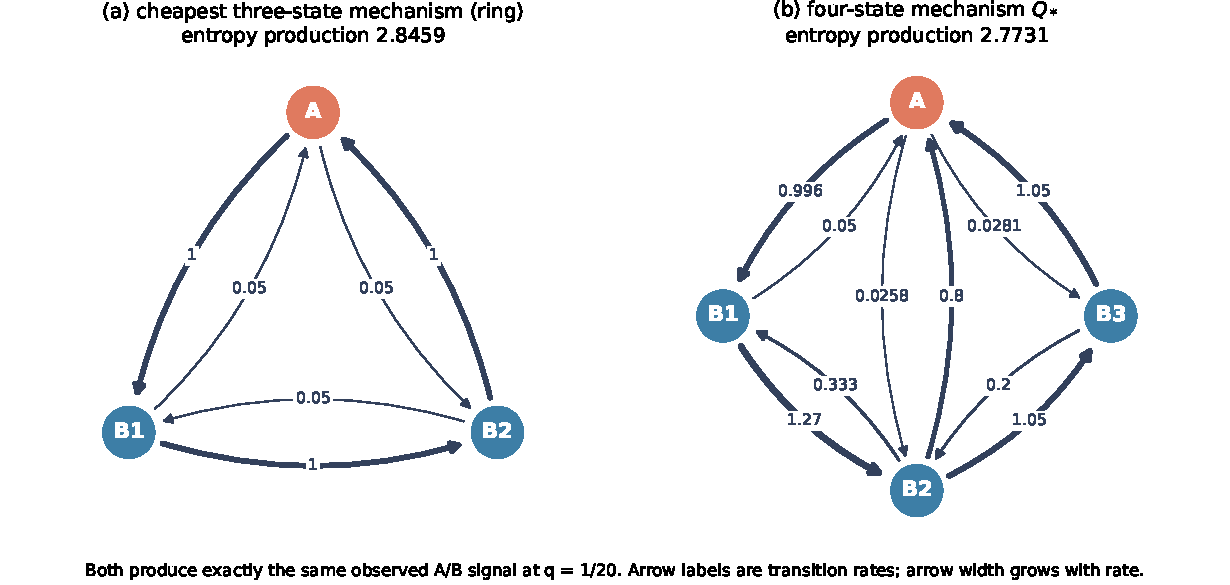
\includegraphics[width=\textwidth]{figures/networks.pdf}
\caption{Two microscopic mechanisms for the same observed signal at
$q=1/20$. Only the label ($A$ or $B$) of the current state is observed.
(a) The three-state ring \eqref{eq:ring}, the unique cheapest three-state
mechanism. (b) The four-state generator \eqref{eq:fourq}. Its observed
signal is identical in every statistical respect, yet it dissipates about
$2.6\%$ less. The pair of edges between $B1$ and $B3$ is absent in both
directions.}
\label{fig:networks}
\end{figure}

\subsection{All two-phase realisations and their minimum}


The denominator in \eqref{eq:target} factors as
\begin{equation}
 p(z)=z^2+2sz+c=(z+\ell)(z+H),\qquad
 \ell=s-\sqrt q,\quad H=s+\sqrt q.
\end{equation}
The numerator at the two poles is nonzero:
$c-b\ell=\ell(H-b)>0$ and $c-bH=H(\ell-b)>0$.
Thus $\widehat f_q$ has reduced degree two. In particular $B$ cannot consist of one
microscopic state. Two total states are insufficient; with three total
states the only possible label allocation is one $A$ and two $B$ states.

Write the two-phase realisation as
\begin{equation}
 S=\begin{pmatrix}-(x+u)&u\\v&-(y+v)\end{pmatrix},\quad
 t=(x,y)^{\mathsf T},\quad \alpha=(a_0,1-a_0).
\end{equation}
Equal exits would give an exponential dwell and are excluded. Relabel to make
$x<y$. Minimality of the degree-two transfer fixes the characteristic
polynomial of $S$ to $p$. Matching trace, determinant and initial density gives
\begin{equation}\label{eq:rectangleformula}
 u=\frac{x^2-2sx+c}{y-x},\quad
 v=-\frac{y^2-2sy+c}{y-x},\quad
 \alpha=\left(\frac{y-b}{y-x},\frac{b-x}{y-x}\right).
\end{equation}
Since $0<b<\ell<H$, the complete nonnegative parameter domain is
\begin{equation}\label{eq:rectangle}
 0\leq x\leq b,\qquad \ell\leq y\leq H.
\end{equation}
Indeed $\alpha t=b$ places $x\leq b\leq y$; then $u>0$, while $v\geq0$
places $y$ between the two roots. Conversely \eqref{eq:rectangleformula}
on this rectangle gives a transient subgenerator and the target transform.

Every boundary face has infinite entropy. If $x=0$, entry into the first
$B$ state has no direct reverse; if $x=b$, the second state exits with
positive flux but has zero entrance flux. At $y=\ell$ or $y=H$, one internal
edge is unidirectional. All states remain used with positive stationary mass.
We may therefore minimise on the open rectangle.

Direct inversion gives
\begin{equation}\label{eq:twomu}
 \mu=\left(\frac{2y/s-1}{y-x},\frac{1-2x/s}{y-x}\right).
\end{equation}
Stationarity gives a common oriented cycle current per visit,
\begin{equation}\label{eq:jcycle}
 j=\alpha_1-\mu_1x
  =\mu_1u-\mu_2v=\mu_2y-\alpha_2
  =\frac{x+y-b-2xy/s}{y-x}>0.
\end{equation}
Thus
\begin{equation}\label{eq:currentaffinity}
 \sigma=\frac{s}{3}j\mathcal A,\qquad
 \mathcal A=\log\frac{\alpha_1uy}{\alpha_2vx}.
\end{equation}

The following change of variables makes the global inequality elementary:
\begin{equation}\label{eq:coordinates}
 a=s-2x,\quad h=2y-s,\quad
 R=\frac{a-D}{a+D},\quad K=\frac{h-D}{h+D}.
\end{equation}
The open domain is $-q<R<q$ and $-\sqrt q<K<\sqrt q$. Substitution in
\eqref{eq:currentaffinity} yields
\begin{equation}\label{eq:mastertwo}
 \sigma=\frac D3\frac{1+RK}{1-RK}
 \log\frac{(1-qR^2)(1-q^2K^2)}{(q^2-R^2)(q-K^2)}.
\end{equation}
In particular $sj=(D^2+ah)/(a+h)=D(1+RK)/(1-RK)>0$,
which also proves the sign asserted in \eqref{eq:jcycle}.

If $RK\geq0$, the current factor is at least one. Each of the two
logarithmic terms is increasing in the relevant square, so their sum is at
least $3\log(1/q)$. Equality requires $R=K=0$.

If $RK<0$, put
\begin{equation}
 u_0=|R|/q,\quad v_0=|K|/\sqrt q,\quad
 \tau=q^{3/2},\quad w=u_0v_0\in(0,1).
\end{equation}
The affinity is
\begin{equation}
 \mathcal A=-2\log\tau+
 \log\frac{1-\tau^2u_0^2}{1-u_0^2}+
 \log\frac{1-\tau^2v_0^2}{1-v_0^2}.
\end{equation}
Expand each last term as
$\sum_{n\geq1}(1-\tau^{2n})u_0^{2n}/n$, or its $v_0$ counterpart.
The coefficients are positive. The arithmetic--geometric mean inequality
at each power gives
\begin{equation}\label{eq:affinitybound}
 \mathcal A\geq2\log\frac{1-\tau^2w}{\tau(1-w)}.
\end{equation}
Let $z=\tau w$, $C=(1-\tau)/(1+\tau)$ and $T=(1+z)/(1-z)>1$.
Then $0<C<CT<1$. Multiplying \eqref{eq:affinitybound} by the current factor
gives
\begin{align}
 \frac{1-z}{1+z}\,2\log\frac{1-\tau z}{\tau-z}
 &=\frac4T\atanh(CT)\nonumber\\
 &>4\atanh C=2\log(1/\tau)=3\log(1/q).
\end{align}
The strict inequality follows from strict increase of $\atanh(v)/v$ on
$(0,1)$, also immediate from its positive power series. Equation
\eqref{eq:mastertwo} proves the global minimum. Equality is possible only
at $R=K=0$, which gives $x=q$, $y=1$, $u=1$, $v=q$ and
$\alpha=(1/s,q/s)$. This is precisely the ring \eqref{eq:ring}.
Its reverse is obtained by exchanging the two $B$ states.

\subsection{Exact four-state realisation and certified gap}

For \eqref{eq:fourq}, the $B$ occupation, entrance and exit vectors are
\begin{equation}\label{eq:fourvectors}
 \mu=(31/36,5/9,41/84),\quad
 \alpha=(683/720,31/1260,3/112),\quad
 t=(1/20,4/5,21/20)^{\mathsf T}.
\end{equation}
All entries are positive. The $B$ submatrix $S_*$ satisfies the exact identities
\begin{equation}\label{eq:fouridentities}
 S_*\one=-t,\quad \mu S_*=-\alpha,\quad
 \mu\one=40/21,\quad \mu t=1,\quad \alpha t=2/21,
\end{equation}
and
\begin{equation}\label{eq:annihilate}
 \left(S_*^2+\frac{21}{10}S_*+\frac{421}{400}I\right)\one=0.
\end{equation}
These identities verify stationarity and full-law matching. In detail, the
survival function $g(\theta)=\alpha e^{\theta S_*}\one$ obeys
$g''+(21/10)g'+(421/400)g=0$, $g(0)=1$ and $g'(0)=-2/21$.
Its density transform is therefore exactly \eqref{eq:target} at $q=1/20$.
Every return to the single $A$ state resets the entrance distribution,
independently of previous visits. Its holding rate is $21/20$.
Consequently all complete visits have the required independent laws.
For a stationary alternating-renewal process, the segment containing time
zero has the standard equilibrium age and residual-life law, which is
determined by the complete dwell laws and the stationary label
probabilities; later segments are independent complete visits. The
stationary fractions agree, so the entire stationary observation process
agrees.

The additional hidden mode is explicit:
\begin{equation}
 \det(zI-S_*)=(z+53/20)
       \left(z^2+\frac{21}{10}z+\frac{421}{400}\right).
\end{equation}
The factor $z+53/20$ cancels from the observed dwell transform. This is an
exact cancellation, rather than a mode made difficult to observe by a small
amplitude. It can nevertheless alter microscopic currents and their entropy
cost.

The five present unoriented edges give
\begin{align}\label{eq:fourentropy}
 \sigma(Q_*)={}&\frac{1141}{3600}\log\frac{683}{31}
 +\frac{529}{3600}\log\frac{560}{31}
 +\frac{17}{100}\log\frac{287}{15}\nonumber\\
 &+\frac{1141}{3600}\log\frac{589}{100}
 +\frac{17}{100}\log\frac{245}{41}.
\end{align}
Rational upper and lower bounds for the logarithms prove
\begin{equation}\label{eq:decimalcert}
 2.773076657<\sigma(Q_*)<2.773076658,
 \qquad \frac{19}{20}\log20-\sigma(Q_*)>0.072869002.
\end{equation}
The certified gap exceeds $2.56\%$ of the three-state minimum. The percentage
describes this competitor, not the maximum possible saving. Appendix
\ref{app:certificate} states the certificate method. This completes the
pointwise comparison in Theorem~\ref{thm:main}.

\begin{figure}[tb]
\centering
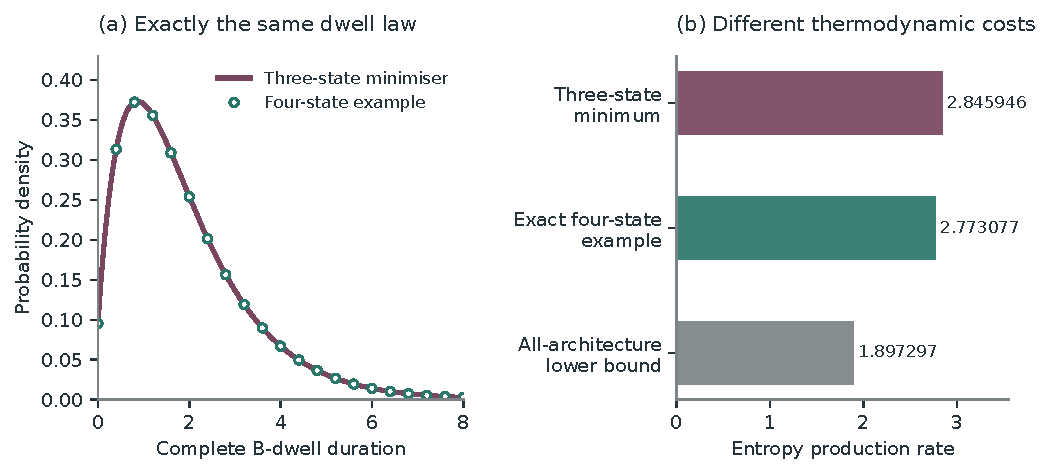
\includegraphics[width=\textwidth]{figures/exact_signal_comparison.pdf}
\caption{Exact observation and different thermodynamic costs at $q=1/20$.
(a) Complete $B$-dwell densities calculated independently from the three-state
and four-state generators coincide; equality is proved for the entire
stationary process, beyond the plotted marginal. (b) The four-state example
lies strictly below the proved three-state minimum. The universal lower bound
from Corollary~\ref{cor:bracket} applies to all finite architectures; its bar
does not represent an attaining model. Rates use the reference time unit of
\eqref{eq:ring}.}
\label{fig:exact}
\end{figure}

\subsection{A strict improvement throughout the family}
\label{sec:allq}

Fix $q$ and write $z_0=s/2$, $\nu =D/s$. Insert a third $B$ phase with exit
rate $z_0$, between the original exit rates $q$ and $1$. Order the phases as
$x,y,w$, with
\begin{equation}\label{eq:splitoccupation}
 t=(q,1,z_0)^{\mathsf T},\qquad
 \mu=(\rho,\rho,\varepsilon),\qquad
 \rho=1/s-\varepsilon/2.
\end{equation}
For a finite parameter $M\geq2$, define
\begin{equation}
 A_0=M/2,\quad B_0=sM/4,\quad C_0=qM/2+\nu ,\quad E_0=sM/4+D/2.
\end{equation}
The internal fluxes per visit are
\begin{align}\label{eq:splitflux}
 &L_{xw}=\varepsilon A_0,\quad L_{wx}=\varepsilon B_0,\quad
 L_{yw}=\varepsilon C_0,\quad L_{wy}=\varepsilon E_0,\nonumber\\
 &L_{xy}=\rho-\varepsilon A_0/2,\qquad
 L_{yx}=q\rho-\varepsilon C_0/2.
\end{align}
Put $S_{ij}=L_{ij}/\mu_i$ for $i\ne j$ and
$S_{ii}=-t_i-\sum_{j\ne i}S_{ij}$. The entrance row is
\begin{equation}\label{eq:splitentry}
 \alpha=\left(\frac{1-q\varepsilon}{s},
              \frac{q(1-\varepsilon)}s,
              \frac{2q\varepsilon}s\right).
\end{equation}
For fixed $M$, sufficiently small positive $\varepsilon$ makes every
off-diagonal rate and every entrance positive. The positive exits ensure
transience, and \eqref{eq:reset} is irreducible.

All these admissible models reproduce $P_q$ exactly. To see this, let
$F(v)=v^2-2sv+c$. Then
\begin{equation}
 F(q)=D,\quad F(1)=-qD,\quad F(z_0)=D^2/4.
\end{equation}
The fluxes satisfy
\begin{equation}\label{eq:splitdrift}
 \sum_{j\ne i}L_{ij}(t_j-t_i)=\mu_iF(t_i).
\end{equation}
At $x$ and $y$ the terms proportional to $A_0$ and $C_0$ cancel; at $w$ the
identity follows from $E_0-B_0=D/2$. Thus $St=c\one-2st$ and $p(S)\one=0$.
Directly, $\mu S=-\alpha$, $\mu\one=2/s$, $\mu t=1$,
$\alpha\one=1$ and $\alpha t=b$. The survival-function argument used for
\eqref{eq:annihilate}, together with reset independence, proves full-law
equality.

It remains to prove a strict entropy decrease. Let $\Psi_M(\varepsilon)$
be the entropy per visit, the expression in braces in
\eqref{eq:phasecost}. As $\varepsilon\downarrow0$, the new phase
disappears and the remaining two phases are the optimal ring. The three
new unoriented edges contribute exactly linear terms in $\varepsilon$,
by homogeneity of $J$. The old edges are smooth near zero. Put
$\Lambda=\log(1/q)$ and $h_+=\Lambda+D$, $h_-=-\Lambda-D/q$.
Their derivatives and the new-edge terms give
\begin{align}\label{eq:splitderivative}
 d_M:=\Psi_M'(0+)
 ={}&h_+(-1-q/s-M/4)
      +h_-(-q-1/2-qM/4)\nonumber\\
 &+J(b,z_0)+J(M/2,sM/4)
       +J(qM/2+\nu ,sM/4+D/2).
\end{align}
The terms linear in $M$ cancel. Expanding the last $J$ term about
$(qM/2,z_0M/2)$ gives the finite limit
\begin{align}\label{eq:splitlimit}
 d_\infty:=\lim_{M\to\infty}d_M
 &=\frac{D^2}{2s}
   \left[3+\log(s/2)-\frac{1+2q}{D}\log(1/q)\right]\nonumber\\
 &=\frac{\nu ^2}{1+\nu }
   \left[3-\frac12\log(1-\nu ^2)-\frac{3\atanh \nu }{\nu }\right].
\end{align}
Its sign is exact, since for $0<\nu <1$ the bracket equals
\begin{equation}\label{eq:negativeseries}
 \sum_{n=1}^{\infty}\frac{1-4n}{2n(2n+1)}\nu ^{2n}<0.
\end{equation}
Choose a finite $M$ with $d_M<0$, then choose a positive admissible
$\varepsilon$ sufficiently small that
$\Psi_M(\varepsilon)<\Psi_M(0)$. This proves
\eqref{eq:allqstrict}. Appendix~\ref{app:explicit} supplies rational formulas
for both parameters and a quantified strict decrease, eliminating any need
for a numerical search in the construction.

The additional decay rate is
\begin{equation}
 \kappa=1+sM/2+\frac{\varepsilon(sM/2+\nu )}{2\rho},
\end{equation}
and $\det(\lambda I-S)=(\lambda+\kappa)p(\lambda)$.
Indeed the target's two poles must be eigenvalues of $S$ and the remaining
root follows from its trace. Since $M\geq2$ gives $\kappa>H$, this mode
is distinct and cancels from the observed law. The construction changes
entropy through an additional mode, rather than by duplicating a state
with unchanged flux ratios.


\section{An architecture-independent lower bound from short dwells}
\label{sec:boundary}

The exact-law optimum remains below the three-state value. To bound it from
below without restricting hidden dimension, we use the initial density of a
complete visit. The next theorem applies to any stationary binary partition;
successive visits may be dependent.

\begin{theorem}[Suppressed immediate returns]\label{thm:boundary}
Let $r>0$ be the stationary entrance intensity into $B$, let $m$ be the mean
complete $B$ dwell under sampling at entrances, and let $f_0=f_B(0)$ be its
right-hand density at zero. If $0<k=mf_0<1$, every finite realisation satisfies
\begin{equation}\label{eq:boundarybound}
 \sigma(Q)>4r\sqrt{1-k}\,\atanh\sqrt{1-k}.
\end{equation}
If $f_0=0$, every compatible finite realisation has infinite entropy production.
\end{theorem}

To prove the theorem, define for every microscopic $B$ state
\begin{equation}\label{eq:palm}
 t_i=\sum_{a\in A}Q_{ia},\quad \mu_i=\frac{\pi_i}{r},\quad
 \alpha_i=\frac{\sum_{a\in A}\pi_aQ_{ai}}r,\quad \beta_i=\mu_it_i.
\end{equation}
Here $\alpha$ and $\beta$ are the entrance and exit distributions at
stationary crossings. Both sum to one. Stationary occupation per entrance
gives $\mu\one=m=\pi(B)/r$, and the killed-chain formula gives
$f_0=\alpha t$. None of these identities requires renewal independence.

Let $\J(p,q)=\sum_i(p_i-q_i)\log(p_i/q_i)$ denote the sum, rather than
the average, of the two relative entropies. Applying log-sum to the boundary
edges at each $B$ state and discarding nonnegative internal contributions gives
\begin{equation}\label{eq:boundarykl}
 \sigma(Q)\geq r\J(\alpha,\beta).
\end{equation}
The Bhattacharyya affinity is bounded by Cauchy--Schwarz:
\begin{equation}\label{eq:affinitycs}
 a=\sum_i\sqrt{\alpha_i\beta_i}
   =\sum_i\sqrt{\mu_i}\sqrt{\alpha_it_i}
   \leq\sqrt{mf_0}.
\end{equation}
Sason's related sharp comparison fixes total variation and defines Jeffreys
divergence as one half of $\J$ \cite{sason}. We require an affinity-constrained
inequality instead, and prove it here without inferring it from that
total-variation comparison.

The function $4d\atanh d$ appearing below is the entropy production of a
single biased link carrying fluxes proportional to $(1\pm d)/2$; functions of
this form also control optimal thermodynamic uncertainty relations
\cite{shiraishi}.

\begin{lemma}[Affinity and symmetric relative entropy]\label{lem:affinity}
For probability vectors $p,q$ with affinity $a=\sum_i\sqrt{p_iq_i}$,
\begin{equation}\label{eq:phi}
 \J(p,q)\geq\Phi(a),\qquad
 \Phi(a)=4\sqrt{1-a^2}\,\atanh\sqrt{1-a^2}.
\end{equation}
The inequality is sharp for each $0<a\leq1$.
\end{lemma}
\begin{proof}
It suffices to consider finite divergence. Put $w_i=(p_i+q_i)/2$,
$u_i=(p_i-q_i)/(p_i+q_i)$ and $z_i=\sqrt{1-u_i^2}$ on indices of positive
total mass. Then $\sum_iw_i=1$, $a=\sum_iw_iz_i$ and
$\J(p,q)=\sum_iw_i\Phi(z_i)$. For $d=\sqrt{1-z^2}$,
\begin{equation}
 \Phi'(z)=-4\left(\frac z d\atanh d+\frac1z\right)<0,
 \qquad
 \Phi''(z)=\frac4{d^3}\left(\frac d{1-d^2}-\atanh d\right)>0.
\end{equation}
The bracket has value zero at $d=0$ and positive derivative
$2d^2/(1-d^2)^2$. Jensen's inequality proves \eqref{eq:phi}; endpoint
cases follow by limits. Equality holds for
$p=((1+d)/2,(1-d)/2)$ and $q=((1-d)/2,(1+d)/2)$.
\end{proof}

Equations \eqref{eq:boundarykl}--\eqref{eq:phi}, and decrease of $\Phi$,
give the non-strict form of \eqref{eq:boundarybound}. Equality would require
zero entropy on all $B$-internal edges. Their stationary fluxes would be
symmetric, so microscopic stationarity would give $\alpha=\beta$. Then
\begin{equation}
 1=(\mu t)^2\leq(\mu\one)\sum_i\mu_it_i^2=mf_0,
\end{equation}
a contradiction. Infinite entropy also satisfies the strict inequality.
Finally, finite entropy requires every used boundary edge to have a reverse;
at least one such edge exists. For its $B$ endpoint both $\alpha_i$ and $t_i$
are positive, forcing $f_0>0$. This proves Theorem~\ref{thm:boundary}.

\begin{corollary}[Unrestricted exact-law bracket]\label{cor:bracket}
For $0<q<1$,
\begin{equation}\label{eq:familybracket}
 \frac23(1-q)\log(1/q)\leq V_\infty(P_q)
 \leq V_4(P_q)<V_3(P_q)=(1-q)\log(1/q).
\end{equation}
At the explicit benchmark,
\begin{equation}\label{eq:benchmarkbracket}
 1.897297106584\ldots
 =\frac{19}{30}\log20
 \leq V_\infty(P_{1/20})
 \leq\sigma(Q_*)=2.773076657835\ldots.
\end{equation}
\end{corollary}
\begin{proof}
The observed statistics are $r=s/3$, $m=2/s$ and $f_0=2q/s$.
Hence $\sqrt{1-mf_0}=D/s$ and $\atanh(D/s)=\tfrac12\log(1/q)$.
Apply Theorem~\ref{thm:boundary} to every exact realisation, then take the
infimum. The explicit four-state model supplies the upper bound.
\end{proof}
The strict inequality for each finite model does not justify replacing the
lower $\leq$ in \eqref{eq:benchmarkbracket} by $<$ after taking the
all-dimension infimum. The endpoints are certified bounds, not confidence
limits or estimates of an optimum.

Equation~\eqref{eq:familybracket} also bounds the benefit of unrestricted
architecture: its relative saving from the minimum-state cost is positive
and at most one third. It fixes both endpoint orders,
\begin{equation}\label{eq:asymptoticorders}
 V_\infty(P_q)=\Theta((1-q)^2)\quad(q\uparrow1),\qquad
 V_\infty(P_q)=\Theta(\log(1/q))\quad(q\downarrow0).
\end{equation}
These are order statements, not determinations of the leading coefficients.

\section{Exact optimisation for three observable statistics}
\label{sec:statistics}

The lower bound has a complete optimality statement when the observed
constraints are precisely $(r,m,f_0)$. It is useful to solve that problem
separately, because it shows exactly what these statistics can and cannot
force thermodynamically.

\begin{theorem}[Sharp cost and nonattainment]\label{thm:statistics}
Fix $r,m,f_0>0$ with $0<rm<1$. Over all finite irreducible stationary
binary-labelled chains with these three $B$ statistics,
\begin{equation}\label{eq:statinf}
 \inf\sigma=
 \begin{cases}
 4r\sqrt{1-mf_0}\,\atanh\sqrt{1-mf_0},&0<mf_0<1,\\
 0,&mf_0\geq1.
 \end{cases}
\end{equation}
The positive infimum is attained by no finite model, but is approached by
three-state models. The zero infimum is attained by a reversible model with
at most three states.
\end{theorem}

\subsection{Positive branch and a fixed-dimension limiting sequence}

Let $d=\sqrt{1-mf_0}\in(0,1)$ and choose $M>d/2$. Set
\begin{equation}\label{eq:sharpvectors}
 \mu=(m/2,m/2),\quad
 \alpha=((1+d)/2,(1-d)/2),\quad
 t=((1-d)/m,(1+d)/m)^{\mathsf T},
\end{equation}
\begin{equation}\label{eq:fastmatrix}
 S_M=\frac1m
 \begin{pmatrix}-(1+2M)&2M+d\\2M-d&-(1+2M)\end{pmatrix},\qquad
 s_A=\frac r{1-rm},\quad
 Q_M=\begin{pmatrix}-s_A&s_A\alpha\\t&S_M\end{pmatrix}.
\end{equation}
All three unoriented edges have positive rates in both directions.
The identities $-S_M\one=t$ and $\mu S_M=-\alpha$ give
\begin{equation}
 \pi_M=(1-rm,rm/2,rm/2).
\end{equation}
The entrance intensity, mean and initial density are respectively
$r$, $m$ and $(1-d^2)/m=f_0$, exactly for every $M$.
Boundary fluxes per visit are $\alpha$ and its reversed vector; the two
internal fluxes are $M+d/2$ and $M-d/2$. Therefore
\begin{equation}\label{eq:fastcost}
 \sigma(Q_M)=r\left\{4d\atanh d+
             d\log\frac{M+d/2}{M-d/2}\right\}.
\end{equation}
The last term tends to zero as $M\to\infty$. Theorem~\ref{thm:boundary}
proves that the limit is the infimum and that no finite model attains it.
Nonattainment is thus immediate from the strict inequality of
Theorem~\ref{thm:boundary}; the new content of Theorem~\ref{thm:statistics}
is that the bound is sharp, and that three states suffice to approach it.


The full dwell law is not constant in this sequence. Direct inversion gives
\begin{equation}\label{eq:fasttransform}
 \widehat f_M(z)=
 \frac{(1-d^2)mz+(1+4M+d^2)}
      {m^2z^2+2m(1+2M)z+(1+4M+d^2)}
 \longrightarrow\frac1{1+mz}.
\end{equation}
The limit is an exponential dwell of mean $m$, whose density at zero is
$1/m$. Every finite member has initial density $(1-d^2)/m<1/m$.
The fast internal mode confines the initial-density discrepancy to a
shrinking time interval. Evaluation of $f(0)$ consequently fails to commute
with this limit. A compactness result for a fixed complete law cannot be
applied to the present constraint set, which is not closed under this
convergence.

For the target statistics of $P_q$, the original ring occurs at $M=1/2$ in
\eqref{eq:fastmatrix}. Raising $M$ lowers its cost while preserving
$(r,m,f_0)$, but changes its dwell transform. It is therefore not an exact-law
competitor. This supplies a direct check on the distinction between
Theorems~\ref{thm:main} and \ref{thm:statistics}.

\begin{figure}[tb]
\centering
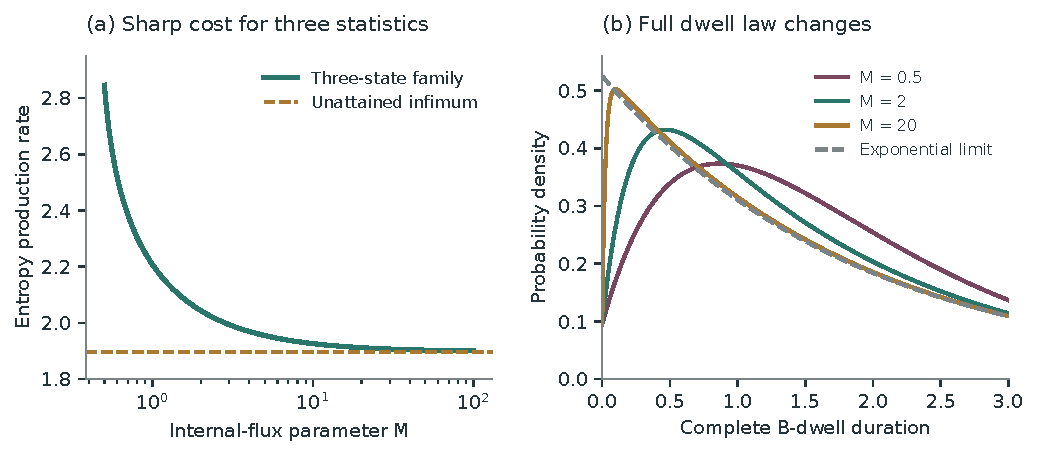
\includegraphics[width=\textwidth]{figures/statistics_nonattainment.pdf}
\caption{The statistics-only optimum has different behaviour from the
exact-law architecture problem. (a) For the $(r,m,f_0)$ of $P_{1/20}$,
\eqref{eq:fastcost} approaches its sharp positive infimum as $M$ grows.
(b) The complete dwell density changes along this family. Its limiting
exponential has a different value at zero despite equality of $f_0$ for
every finite $M$. Thus this sequence cannot establish fixed-law
nonattainment. The time and rate units are those of Figure~\ref{fig:exact}.}
\label{fig:statistics}
\end{figure}

\subsection{Zero branch}

When $k=mf_0=1$, a two-state chain with rates $s_A=r/(1-rm)$ and $1/m$
is reversible and has the required statistics. When $k>1$, put
\begin{equation}
 w_2=\frac1{4k-3},\quad w_1=1-w_2,\quad
 \mu=m(w_1,w_2),\quad
 t=\left(\frac1{2m},\frac{2k-1}{m}\right)^{\mathsf T}.
\end{equation}
Let $S=-\diag(t)$ and $\alpha_i=\mu_it_i$, using the same reset rate
$s_A$. One checks $\alpha\one=1$, $\mu\one=m$ and $\alpha t=f_0$.
Every boundary stationary flux equals its reverse; there are no internal
$B$ edges. The resulting three-state star is irreducible and reversible.
This proves the remaining part of Theorem~\ref{thm:statistics}.

\section{How large can the architecture saving be?}
\label{sec:numerics}

The theorems above leave a gap at $q=1/20$ between the architecture-independent
floor $1.8973$ and the four-state cost $2.7731$. This section narrows the
upper end with a further exact competitor and reports numerical exploration
of the remaining questions. Only Proposition~\ref{prop:improved} is a proved
statement; the rest is discovery evidence obtained by local optimisation from
many random starts, and it is not used in any proof.

\begin{proposition}[Improved exact four- and five-state competitors]\label{prop:improved}
At $q=1/20$ the rational generator, with the first state labelled $A$,
\begin{equation}\label{eq:improved}
 Q_\sharp=
 \begin{pmatrix}
 -\frac{21}{20}&\frac{483}{20000}&\frac{974299}{28880000}&\frac{28652249}{28880000}\\[2pt]
 \frac{134}{125}&-\frac{93181}{75375}&\frac{12379}{75375}&0\\[2pt]
 \frac{1541}{2000}&\frac{1869}{2000}&-\frac{2969283}{1444000}&\frac{507263}{1444000}\\[2pt]
 \frac{97}{2000}&0&\frac{3812009}{2888000}&-\frac{3952077}{2888000}
 \end{pmatrix}
\end{equation}
realises $P_{1/20}$ exactly and has
\begin{equation}
 \sigma(Q_\sharp)=2.765997710528\ldots,\qquad
 V_3(P_{1/20})-\sigma(Q_\sharp)>0.0799479,
\end{equation}
a saving of $2.81\%$. The rational five-state generator
\begin{equation}\label{eq:five}
 Q_5=
 \begin{pmatrix}
 -\frac{21}{20}&\frac{1113}{80000}&\frac{1701}{80000}&\frac{50952901}{51480000}&\frac{129029}{5148000}\\[2pt]
 \frac{139}{125}&-\frac{63247}{46500}&\frac{11539}{46500}&0&0\\[2pt]
 \frac{463}{500}&\frac{897}{1000}&-\frac{1257919}{469000}&0&\frac{100733}{117250}\\[2pt]
 \frac{6}{125}&0&0&-\frac{246223}{160875}&\frac{238501}{160875}\\[2pt]
 \frac{1383}{2000}&0&\frac{2323}{1000}&\frac{33907}{46800}&-\frac{54683}{14625}
 \end{pmatrix}
\end{equation}
also realises $P_{1/20}$ exactly, with
\begin{equation}
 \sigma(Q_5)=2.746985402969\ldots,\qquad
 V_3(P_{1/20})-\sigma(Q_5)>0.0989602,
\end{equation}
a saving of $3.48\%$. Consequently
$1.8973\leq V_\infty(P_{1/20})\leq V_5(P_{1/20})\leq2.7469855$ and
$V_4(P_{1/20})\leq2.7659978$.
\end{proposition}
\begin{proof}
The verification follows Section~\ref{sec:main} line by line, in exact rational
arithmetic. The rows sum to zero, the off-diagonal entries are nonnegative and
the only zeros form a reciprocal pair. With $S$ the $B$ block,
$t=-S\one$, $\alpha$ the normalised first row and $\mu=\alpha(-S)^{-1}$,
one has $\alpha\one=1$, $\alpha t=2/21$, $\mu\one=40/21$, $\mu t=1$, $\mu>0$
and $(S^2+\tfrac{21}{10}S+\tfrac{421}{400}I)\one=0$. As for
\eqref{eq:annihilate}, these identities and the single reset state give the
complete law $P_{1/20}$. The characteristic polynomial is
$\det(zI-S)=(z+\tfrac{4459837153}{1741464000})(z^2+\tfrac{21}{10}z+\tfrac{421}{400})$,
so again one hidden mode cancels. The cost is a sum over five edges of terms
$(x-y)\log(x/y)$ with rational $x,y$, enclosed by the series of
Appendix~\ref{app:certificate}. The same identities hold for $Q_5$ with its
four-state $B$ block, whose zeros form three reciprocal pairs; there
$\det(zI-S)$ is the product of

$z^2+\tfrac{21}{10}z+\tfrac{421}{400}$ and
$z^2+\tfrac{134945227969}{18711693000}z+\tfrac{156924372390977}{14033769750000}$,
so two hidden modes cancel, and the cost is a sum over seven edges.
The stationary vector of $Q_\sharp$ is
\[
 \pi_\sharp=\Bigl(\frac13,\frac{3650219496}{22299185765},
 \frac{27820291057}{133795114590},\frac{39475135027}{133795114590}\Bigr).
\]
Both scripts print the exact stationary vectors and certify the rational
enclosures
\[
 2.765997710527<\sigma(Q_\sharp)<2.765997710529,\qquad
 2.746985402969<\sigma(Q_5)<2.746985402970.
\]

 The scripts \texttt{extension/verify\_improved.py} and
\texttt{extension/verify\_five.py} perform every step with the Python standard
library.

\end{proof}

\paragraph{The four-state optimum.}
By the reset lemma (Appendix~\ref{app:reset}), every four-state exact
realisation can be replaced, at no greater cost, by one with a single $A$
state and at most three $B$ states. Those with at most two $B$ states cost at
least $V_3(P_{1/20})$, so a four-state minimiser below $V_3$ may be sought
among models with one $A$ and three $B$ states. We searched this class
from random starts, both over the stratum on which $p(S)\one=0$, which contains
$Q_*$ and $Q_\sharp$ and is mapped to its reversed counterpart
$\alpha\,p(S)=0$ by time reversal, and, independently, over all three-phase
representations constrained only by the first three derivatives
$f(0),f'(0),f''(0)$ of the dwell density. The second problem is a relaxation of
the exact-law problem, so its minimum cannot exceed $V_4(P_{1/20})$. Both
searches returned the same best local value, $2.765996$, with one reciprocal
pair of internal edges tending to zero. $Q_\sharp$ is a rational rounding of
the best local solution found, and its cost is within $2\times10^{-6}$ of it.
The coincidence of the two searches motivates, but does not certify, the
conjecture that $V_4(P_{1/20})=2.76599\ldots$, attained on the boundary stratum
on which one internal edge pair is absent. A certified global optimisation
would be needed to turn this into a theorem. The searches used SLSQP with
150--400 random starts per stratum, enumerated every pattern of up to three
absent edge pairs, and accepted only solutions with constraint residuals
below $10^{-9}$.

\paragraph{The whole family.}
Table~\ref{tab:grid} repeats the search for other values of $q$.
Among the sampled values, the largest relative saving found, about $6\%$, is
at the smallest $q=0.01$ (strong driving), and the savings found become very
small as $q$ approaches one, where the ring approaches equilibrium. The data
are consistent with, but do not establish, a vanishing relative saving as
$q\uparrow1$. The proved floor stays well below every four-state value, so the
table does not indicate whether larger architectures could approach it.
\begin{table}[tb]\centering\small
\caption{Numerical exploration of the four-state optimum across the family. $V_3$ and the floor are proved; the third column is the best exact four-state cost found by local optimisation from random starts, so it is an upper estimate of $V_4$ and the saving is a lower estimate. For $q\geq0.5$ the savings found are tiny and not monotone in $q$, so these rows are inconclusive about the size of the saving; Theorem~\ref{thm:main} guarantees that every saving is positive.}
\label{tab:grid}
\begin{tabular}{@{}rcccc@{}}\toprule
$q$ & $V_3$ (proved) & best four-state cost found & saving found & floor $\tfrac23V_3$ (proved)\\\midrule
0.01 & 4.55912 & 4.29941 & 0.25970 (5.7\%) & 3.03941\\
0.05 & 2.84595 & 2.76600 & 0.07995 (2.8\%) & 1.89730\\
0.1 & 2.07233 & 2.03755 & 0.03477 (1.7\%) & 1.38155\\
0.2 & 1.28755 & 1.27774 & 0.00981 (0.76\%) & 0.85837\\
0.3 & 0.84278 & 0.83955 & 0.00323 (0.38\%) & 0.56185\\
0.5 & 0.34657 & 0.34657 & $4.7\times10^{-6}$ (0.0013\%) & 0.23105\\
0.7 & 0.10700 & 0.10699 & $9.8\times10^{-6}$ (0.0091\%) & 0.07133\\
0.9 & 0.01054 & 0.01054 & $6.4\times10^{-8}$ (0.00061\%) & 0.00702\\
\bottomrule\end{tabular}\end{table}


\paragraph{Does a fifth state help?}
The same search with four hidden $B$ states, over the stratum $p(S)\one=0$,
returned $2.746985$, and the rational rounding $Q_5$ of
Proposition~\ref{prop:improved} certifies a cost within $10^{-6}$ of this value.
A search with five hidden $B$ states, from random interior starts only,
returned $2.739391$. The successive best costs found,
\[
 2.845946\ (n=3),\quad 2.765996\ (n=4),\quad 2.746985\ (n=5),\quad
 2.739391\ (n=6),
\]
decrease with shrinking steps $0.080$, $0.019$ and $0.0076$. Only the first is
a proved minimum and the others are upper estimates, so this is not evidence
of a limit. It does suggest that each added hidden state lowers the best
achievable cost further, which bears on the question of \cite{aznagulov} whether the
selected state count diverges as the price per state tends to zero. If it
does, no finite architecture attains $V_\infty(P_{1/20})$.

\paragraph{Can more local statistics sharpen the floor?}
A natural attempt to raise the lower bound adds further short-time
statistics to $(r,m,f_0)$. Numerical minimisation suggests that the first
derivative $f'(0)$ does not help: with three hidden $B$ states and the exact
values of $r,m,f_0$ and $f'(0)$ for $P_{1/20}$, the best local cost found came
within $3\times10^{-6}$ of the floor $1.8973$. If that local solution is close
to the global one, $f'(0)$ alone cannot materially raise the floor. Matching
$f''(0)$ as well raised the best three-hidden-state cost found to the
four-state value $2.766$, but runs with more hidden states did not reach the
feasibility tolerance, so we draw no conclusion from them about larger
architectures.


\section{Interpretation, verification and limits}

\label{sec:discussion}

The exact architecture comparison has a direct inference consequence. Suppose
the true physical generator is $Q_*$. An observer with its entire stationary
binary signal can fit a three-state model perfectly. Minimising dissipation
over every such three-state fit gives a value larger than the physical
dissipation of $Q_*$. Thus statistical adequacy and the fewest possible hidden
states do not make that restricted minimum a valid architecture-independent
lower bound. This conclusion concerns the exact-law optimisation. It does
not invalidate lower bounds that optimise over a proved complete class or
over a sufficiently broad relaxation of the observations.

The structural reason is visible in \eqref{eq:annihilate}: a microscopic
mode can cancel from the observed dwell law while changing the current
distribution. Reducing a transfer function to its smallest linear
realisation does not preserve the nonlinear flux functional
\eqref{eq:epr}. Nor does an arbitrary similarity transformation preserve
nonnegative transition rates. The proof avoids both assumptions by checking
all two-phase models analytically and constructing a positive larger model
directly.

The short-dwell bound quantifies a complementary obstruction. If
$mf_0<1$, the entrance and exit distributions of hidden states must differ.
Their affinity is bounded away from one, forcing entropy at the observed
boundary regardless of hidden dimension. The result detects a thermodynamic
cost even without independent visits. It uses an infinitesimal property of a
complete dwell density, however. Estimating $f_0$ from finite-resolution or
finite-duration data requires further assumptions and analysis. In
single-channel recording this is the classical missed-events problem: events
shorter than the dead time are not detected and distort the apparent dwell
distributions near zero \cite{hjc}. We supply no
statistical coverage statement and no experimental calibration. Units are
fixed only by the time scale: if the rate-one transitions of \eqref{eq:ring}
occurred at $10^3\,\mathrm{s}^{-1}$, every cost above would be multiplied by
$10^3$, so the explicit saving at $q=1/20$ would be about
$73\,k_B\,\mathrm{s}^{-1}$.

All principal claims are analytic. Computational exploration located the
simple rational competitor on a branch satisfying $p(S)\one=0$; the
full-family improvement is established analytically. This branch
does not exhaust higher-dimensional representations \cite{aznagulov}.
Exhaustiveness is unnecessary for an upper-bound competitor; we do not use
it to claim a four-state or unrestricted minimum. The final certificate
contains rational generators, stationary vectors, polynomial identities and
rational enclosures of logarithms. Supporting checks cover the complete
two-phase parametrisation, random binary partitions without renewal
independence, the information inequality and the sharp limiting families.
Numerical optimisations are recorded as discovery calculations, including
failed runs, and are excluded from the logical certificate.

The unresolved problem is precise. We have proved a strict drop from the
smallest exact architecture and a positive lower bound valid over all finite
architectures. We have not determined $V_4(P_{1/20})$, $V_\infty(P_{1/20})$
or whether a finite model attains the latter. The fixed-statistics
nonattainment theorem does not answer the fixed-law question. A further
global certificate or an exactly compatible improving sequence is needed.
These limits leave a complete stand-alone result: one extra hidden state can
reduce the least physical cost of an unchanged stochastic signal, and the
initial dwell density admits a sharp universal cost formula with a fully
resolved attainment distinction.

\paragraph{Code and verification materials.}
The accompanying archive contains the manuscript source, exact certificates,
reproduction scripts, figure code, numerical discovery record and bounded
prior-art audit. The central rational certificate uses the Python standard
library. Additional diagnostics and figures use NumPy, SciPy and Matplotlib.
Internal independent checking is documented separately; it is not external
peer review or proof-assistant verification.

\paragraph{Availability.}
This version (1.0.0-candidate) is archived at Zenodo, DOI
\href{https://doi.org/10.5281/zenodo.23721621}{10.5281/zenodo.23721621}, with source repository
\url{https://github.com/ipitchford/hidden-architecture-exact-signal} and release page
\url{https://evidencepress.org/releases/hidden-architecture-exact-signal/}. Text and figures are
released under CC0-1.0 and code under the MIT licence.

\appendix
\section{Reset replacement and the scope of the three-state theorem}
\label{app:reset}

\begin{lemma}[Reset replacement]\label{lem:reset}
Let a finite stationary chain realise an alternating-renewal law whose $A$
dwell is $\Exp(s)$. Replacing its whole $A$ block by one reset state, as
below, gives a chain with the same complete observed law and no larger
entropy production. Consequently every exact realisation of $P_q$ with at
most two $B$ states, and any number of $A$ states, has cost at least
$(1-q)\log(1/q)$.
\end{lemma}
A single $B$ state would give an exponential $B$ dwell, which $P_q$ excludes,
so the lemma covers all realisations with exactly two $B$ states. The
reduction is a full-law corollary of the stationary-flux merge of Skinner and
Dunkel \cite[Supplementary Lemma 2]{skinner_wait}; it is included with
attribution.

\begin{proof}
Keep $S=Q_{BB}$ and set
\begin{equation}
 t_i=\sum_{a\in A}Q_{ia},\quad
 r=\sum_{a,i}\pi_aQ_{ai}=\sum_i\pi_it_i,\quad
 \alpha_i=r^{-1}\sum_a\pi_aQ_{ai}.
\end{equation}
Replace the whole $A$ block by one state with exit rate $s$ and entrance
distribution $\alpha$ into $B$. The resulting generator is
\eqref{eq:reset}. It is irreducible and has stationary distribution
$(\pi(A),\pi_B)$ because $\pi(A)=r/s$ and
$r\alpha+\pi_BS=0$. Its $B$ dwell density is the original
$\alpha e^{\theta S}t$. The single reset state makes complete visits independent.
Since independence is part of the target law, matching the two dwell laws and
stationary fractions matches the full stationary process.

$B$-internal fluxes are unchanged. $A$-internal entropy is discarded, and each
new boundary flux pair is a sum of old pairs. The log-sum inequality gives
\begin{equation}
 J\left(\sum_a x_a,\sum_a y_a\right)\leq\sum_aJ(x_a,y_a),
\end{equation}
so entropy cannot increase. The original chain need not be lumpable; this is
an observationally equivalent replacement. Without renewal independence,
resetting can destroy dependencies and does not generally preserve the
observed law. Applying the reduction to $P_q$ with at most two $B$ states
then invoking the proved three-state minimum gives the claimed extension.
\end{proof}

\section{Explicit finite parameters for the full-family improvement}
\label{app:explicit}

The construction in Section~\ref{sec:allq} can be made fully explicit.
Using $\nu =D/s$ and $z_0=s/2$, define
\begin{align}
 \eta&=\frac{\nu ^4}{2(1+\nu )},\nonumber\\
 C_*&=\left(q+z_0+\nu +\frac D2\right)
       \left(\frac \nu q+\frac{D}{2z_0}\right)^2,\qquad
 M=2+\frac{4C_*}{\eta}.
\end{align}
All are positive rational functions of $q$. The first term of
\eqref{eq:negativeseries} gives $d_\infty\leq-\eta$.
For the symmetric-divergence Hessian,
\begin{equation}\label{eq:hessian}
 v^{\mathsf T}\nabla^2J(x,y)v
 =(x+y)\left(\frac{v_1}{x}-\frac{v_2}{y}\right)^2.
\end{equation}
Apply the integral Taylor remainder to the last term of
\eqref{eq:splitderivative}, from the baseline $(qM/2,z_0M/2)$
with offset $(\nu ,D/2)$. Along this segment the coordinates are at least
their baseline values, and their sum is at most
$(M/2)(q+z_0+\nu +D/2)$ because $M/2\geq1$.
Equation~\eqref{eq:hessian} bounds the second directional derivative by
$2C_*/M$. Therefore
\begin{equation}
 0\leq d_M-d_\infty\leq C_*/M<\eta/4,
 \qquad d_M<-3\eta/4.
\end{equation}

Now put
\begin{align}
 B_*&=4\left[
       \left(q+\frac s2\right)^2+
       \left(1+\frac s2\right)^2+
       \left\{\frac s2\left(M+2+\frac \nu q\right)\right\}^2
       \right],\nonumber\\
 \varepsilon_0&=\frac{2q}{s[q(M+2)+2\nu ]},\qquad
 \varepsilon=\min\left\{\varepsilon_0,\frac{\eta}{2B_*}\right\}>0.
\end{align}
For $0\leq v\leq\varepsilon_0$, each of the six old directed fluxes
remains at least half its value at zero. All decrease with $v$, and the
sum of each old pair is initially one. The sums of their absolute slopes
relative to their respective initial values are
\begin{equation}
 q+s/2,\qquad 1+s/2,\qquad (s/2)(M+2+\nu /q).
\end{equation}
Equation~\eqref{eq:hessian} consequently gives
$\Psi_M''(v)\leq B_*$. The new-edge terms are exactly linear.
Taylor's theorem yields
\begin{equation}
 \Psi_M(\varepsilon)-\Psi_M(0)
 \leq d_M\varepsilon+\frac{B_*}{2}\varepsilon^2
 <-\frac{\eta\varepsilon}{2}<0.
\end{equation}
All rates are finite and strictly positive, and
\begin{equation}
 \sigma(Q)<(1-q)\log(1/q)-\frac{s\eta\varepsilon}{6}.
\end{equation}
For rational $q$, every chosen parameter and generator entry is rational.
These choices are deliberately conservative and only prove existence. The
certified saving they give is extremely small: $\varepsilon$ is of order
$10^{-20}$ at $q=10^{-4}$ and about $6\times10^{-32}$ at $q=0.999$. The quantitative
size of the four-state saving is better judged from the explicit example
\eqref{eq:fourq} and from the numerical exploration in
Section~\ref{sec:numerics}.


\section{Exact logarithm and polynomial certificates}
\label{app:certificate}

For rational $x>0$, put $v=(x-1)/(x+1)$. When $x>1$,
\begin{equation}\label{eq:logseries}
 \log x=2\sum_{j=0}^{N-1}\frac{v^{2j+1}}{2j+1}+R_N,
 \qquad
 0<R_N\leq\frac{2v^{2N+1}}{(2N+1)(1-v^2)}.
\end{equation}
All quantities on the right are rational. Reciprocal arguments or dyadic
range reduction handle other positive rationals. The shipped certificate
reduces each argument dyadically and then uses $N=72$ series terms, giving
rational enclosures of width below $10^{-24}$; the enclosing rational
endpoints are printed in the certificate output. Applying these bounds to

the five terms in \eqref{eq:fourentropy} and to $(19/20)\log20$ certifies
\eqref{eq:decimalcert} without a floating-point comparison. Generator row
sums, stationary balance, the annihilator \eqref{eq:annihilate} and the
transfer-polynomial cancellation are checked with rational arithmetic.

The two-phase numerical diagnostic independently calculates costs from the
full stationary fluxes, the cycle-current expression and
\eqref{eq:mastertwo}, including parameters near equilibrium. These checks
guard the algebraic transcription; the series inequality in the text, rather
than a parameter grid, proves global optimality.

\begin{thebibliography}{99}
\bibitem{ehrich}
Ehrich, J. (2021). Tightest bound on hidden entropy production from partially
observed dynamics. \emph{Journal of Statistical Mechanics: Theory and
Experiment, 2021}(8), 083214.
\url{https://doi.org/10.1088/1742-5468/ac150e}.

\bibitem{nitzan}
Nitzan, E., Ghosal, A., \& Bisker, G. (2023). Universal bounds on entropy
production inferred from observed statistics. \emph{Physical Review Research,
5}(4), 043251. \url{https://doi.org/10.1103/PhysRevResearch.5.043251}.

\bibitem{skinner_wait}
Skinner, D. J., \& Dunkel, J. (2021). Estimating entropy production from waiting
time distributions. \emph{Physical Review Letters, 127}(19), 198101.
\url{https://doi.org/10.1103/PhysRevLett.127.198101}.

\bibitem{skinner_improved}
Skinner, D. J., \& Dunkel, J. (2021). Improved bounds on entropy production in
living systems. \emph{Proceedings of the National Academy of Sciences,
118}(18), e2024300118. \url{https://doi.org/10.1073/pnas.2024300118}.

\bibitem{aznagulov}
Aznagulov, M. (2026). \emph{Thermodynamic realizability of hidden Markov
processes: Attainment, observable certificates, and the price of architecture}
[Preprint, version 1]. arXiv.
\url{https://arxiv.org/abs/2609.14623v1}.

\bibitem{ep_floor}
Anonymous. (2026, October 3). \emph{An architecture-independent dissipation
floor for alternating-renewal observations} (Version 1.1) [Unrefereed research
candidate]. Evidence Press. \url{https://doi.org/10.5281/zenodo.23118474}.


\bibitem{sason}
Sason, I. (2015). Tight bounds for symmetric divergence measures and a refined
bound for lossless source coding. \emph{IEEE Transactions on Information
Theory, 61}(2), 701--707. \url{https://doi.org/10.1109/TIT.2014.2387065}.

\bibitem{martinez}
Mart\'inez, I. A., Bisker, G., Horowitz, J. M., \& Parrondo, J. M. R. (2019).
Inferring broken detailed balance in the absence of observable currents.
\emph{Nature Communications, 10}(1), 3542.
\url{https://doi.org/10.1038/s41467-019-11051-w}.

\bibitem{vdm_prx}
van der Meer, J., Ertel, B., \& Seifert, U. (2022). Thermodynamic inference
in partially accessible Markov networks: A unifying perspective from
transition-based waiting time distributions. \emph{Physical Review X, 12}(3),
031025. \url{https://doi.org/10.1103/PhysRevX.12.031025}.

\bibitem{harunari}
Harunari, P. E., Dutta, A., Polettini, M., \& Rold\'an, \'E. (2022). What to
learn from a few visible transitions' statistics? \emph{Physical Review X,
12}(4), 041026. \url{https://doi.org/10.1103/PhysRevX.12.041026}.

\bibitem{hartich}
Hartich, D., \& Godec, A. (2021). Emergent memory and kinetic hysteresis in
strongly driven networks. \emph{Physical Review X, 11}(4), 041047.
\url{https://doi.org/10.1103/PhysRevX.11.041047}.

\bibitem{vdm_prl}
van der Meer, J., Degünther, J., \& Seifert, U. (2023). Time-resolved
statistics of snippets as general framework for model-free entropy
estimators. \emph{Physical Review Letters, 130}(25), 257101.
\url{https://doi.org/10.1103/PhysRevLett.130.257101}.

\bibitem{deguenther}
Degünther, J., van der Meer, J., \& Seifert, U. (2024). Fluctuating entropy
production on the coarse-grained level: Inference and localization of
irreversibility. \emph{Physical Review Research, 6}(2), 023175.
\url{https://doi.org/10.1103/PhysRevResearch.6.023175}.

\bibitem{shiraishi}
Shiraishi, N. (2021). Optimal thermodynamic uncertainty relation in Markov
jump processes. \emph{Journal of Statistical Physics, 185}(3), 19.
\url{https://doi.org/10.1007/s10955-021-02829-8}.

\bibitem{benvenuti}
Benvenuti, L., \& Farina, L. (2004). A tutorial on the positive realization
problem. \emph{IEEE Transactions on Automatic Control, 49}(5), 651--664.
\url{https://doi.org/10.1109/tac.2004.826715}.

\bibitem{ocinneide}
O'Cinneide, C. A. (1990). Characterization of phase-type distributions.
\emph{Communications in Statistics. Stochastic Models, 6}(1), 1--57.
\url{https://doi.org/10.1080/15326349908807134}.

\bibitem{hjc}
Hawkes, A. G., Jalali, A., \& Colquhoun, D. (1990). The distributions of the
apparent open times and shut times in a single channel record when brief
events cannot be detected. \emph{Philosophical Transactions of the Royal
Society of London. Series A, 332}(1627), 511--538.
\url{https://doi.org/10.1098/rsta.1990.0129}.

\bibitem{owen}
Owen, J. A., Kolchinsky, A., \& Wolpert, D. H. (2019). Number of hidden states
needed to physically implement a given conditional distribution.
\emph{New Journal of Physics, 21}(1), 013022.
\url{https://doi.org/10.1088/1367-2630/aaf81d}.
\end{thebibliography}
\end{document}
